\documentclass[10pt,a4paper]{article}
\usepackage[utf8]{inputenc}
\usepackage[T1]{fontenc}
\usepackage{mathptmx}            % Times-like font
\usepackage[a4paper,left=2cm,right=2cm,top=1.5cm,bottom=1.5cm]{geometry}
\usepackage{graphicx}
\usepackage{booktabs}
\usepackage{enumitem}
\usepackage{xcolor}
\usepackage{microtype}
\usepackage[hidelinks]{hyperref}
\usepackage{titlesec}

\setlength{\parindent}{0pt}
\setlength{\parskip}{4pt}
\setlist{nosep,leftmargin=*}
\titleformat{\section}{\normalfont\large\bfseries}{\thesection}{0.6em}{}
\titleformat{\subsection}{\normalfont\normalsize\bfseries}{\thesubsection}{0.6em}{}
\titlespacing*{\section}{0pt}{8pt}{3pt}
\titlespacing*{\subsection}{0pt}{6pt}{2pt}

% Text that was highlighted yellow in the Word version is shown in red.
\newcommand{\red}[1]{\textcolor{red}{#1}}

\begin{document}

\begin{center}
{\Large\bfseries Movie Rec Hub: a Microservice Movie Recommendation Platform}\\[3pt]
PSIA Project Report - Group 34\\[3pt]
Group members: 109358 - Gon\c{c}alo Torcato, 120202 - Sara Nascimento, 120232 - Sofia Rodrigues\\[3pt]
Video: link
\end{center}

\section*{1 Introduction}

Movie Rec Hub is a web application where users browse movies, write reviews, organise movies into lists and receive personalised recommendations. The recommendations are produced by a large language model (LLM) that takes into account each user's lists, reviews and favourite genres.

The application is built as a set of Spring Boot microservices, each with its own PostgreSQL database. It runs locally with Docker Compose and in the Google Cloud on a Kubernetes cluster created with Terraform and configured with Ansible. The system also includes an LLM-based recommendation service and a monitoring stack with Prometheus and Grafana. As an advanced feature, the application keeps its state across a full shutdown of the infrastructure.

This report presents the design and deployment of the base system, including monitoring (Section~2), the persistent state feature (Section~3) and an evaluation of throughput and latency as the number of clients grows (Section~4). The video linked above shows the system running in the cloud.

\section*{2 System Design and Architecture}

\begin{center}
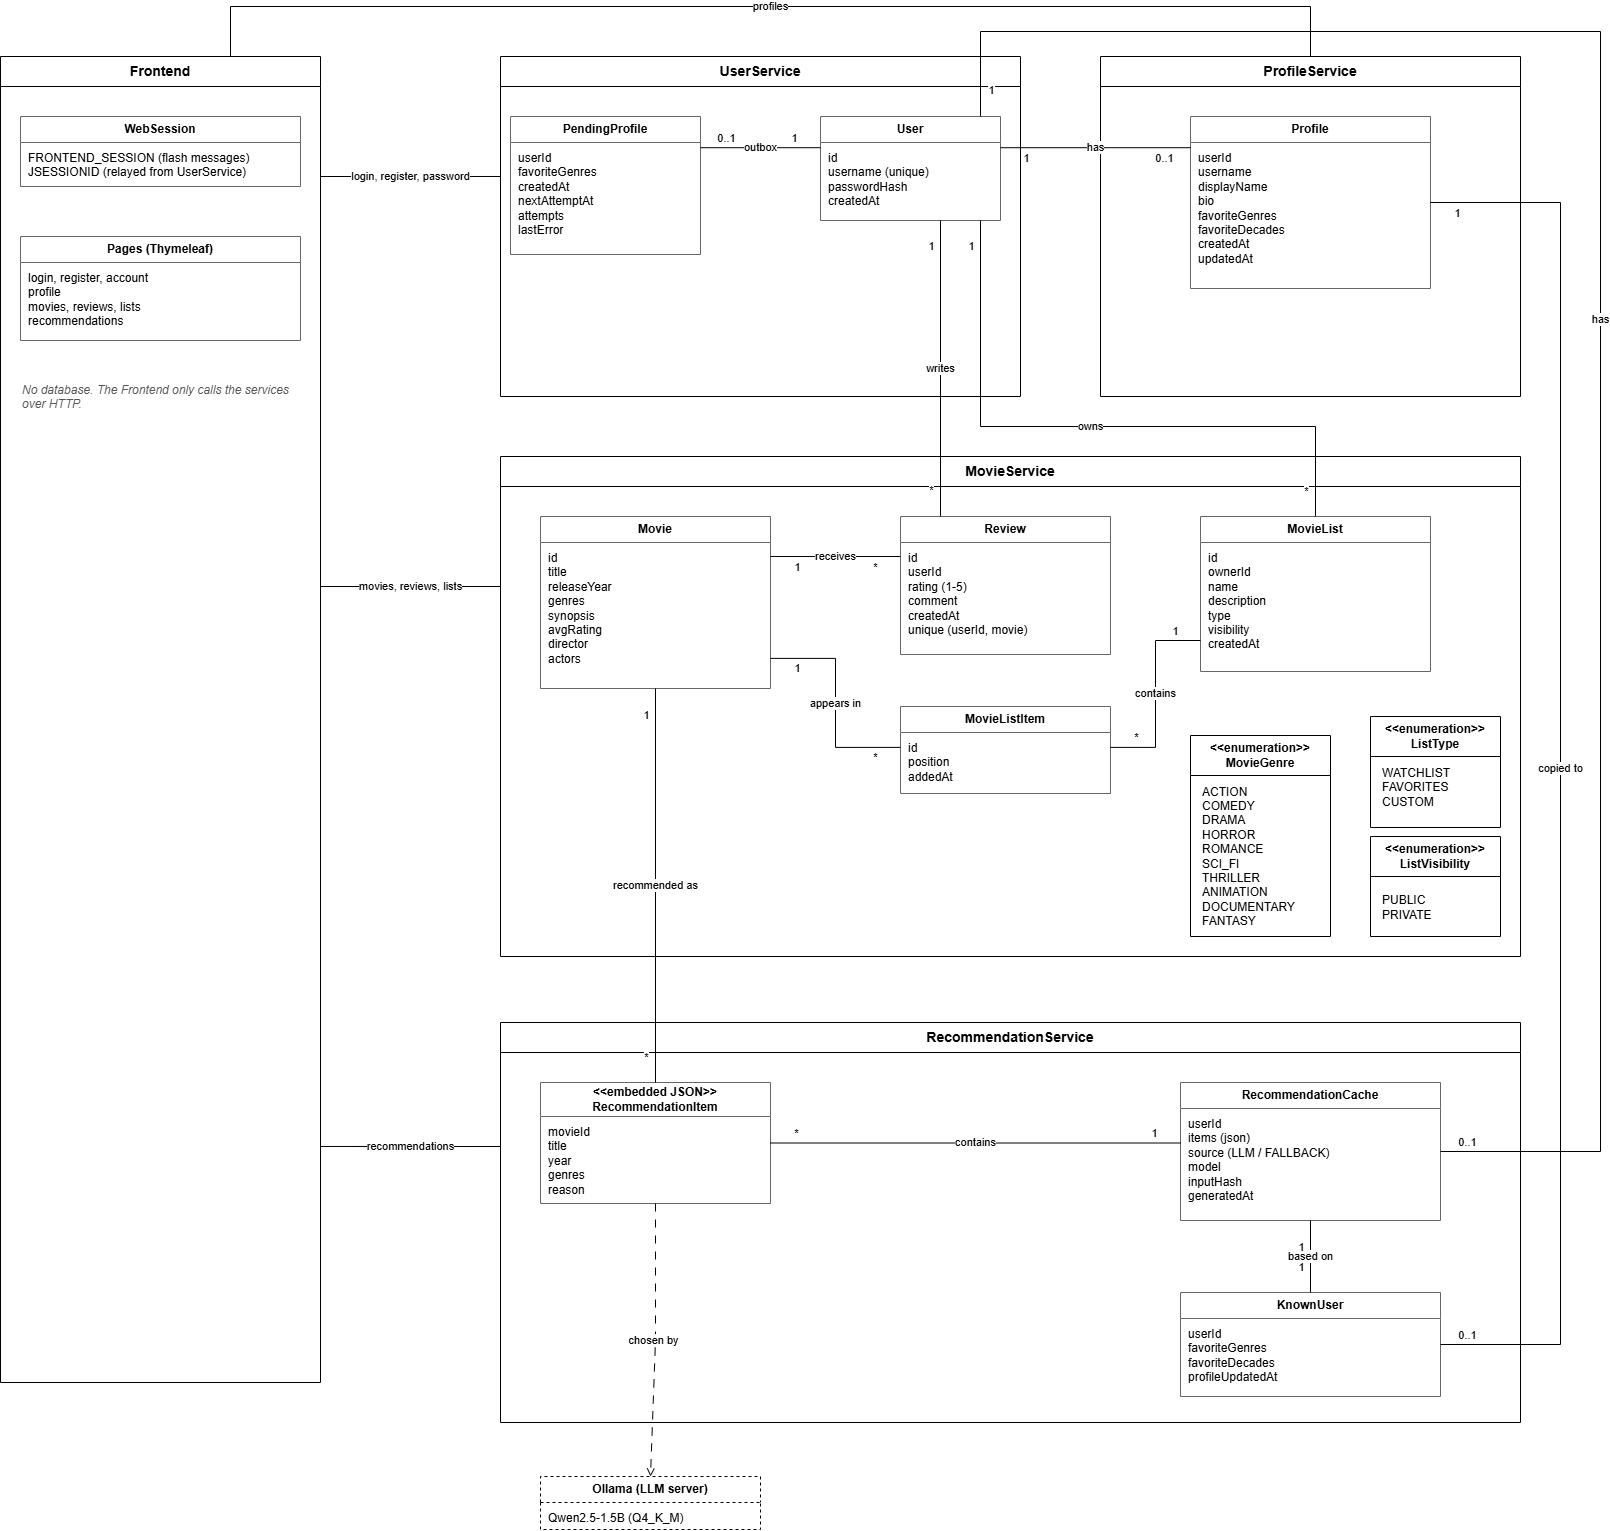
\includegraphics[width=0.8\linewidth]{DomainModel.png}\\[2pt]
\emph{Fig. 1. Architecture of Movie Rec Hub.}
\end{center}

The system is composed of five services that communicate through REST APIs:
\begin{itemize}
  \item \textbf{Frontend:} the only entry point for users. It renders the web pages and calls the other services.
  \item \textbf{UserService:} accounts, login and sessions.
  \item \textbf{ProfileService:} user profiles, favourite genres and decades.
  \item \textbf{MovieService:} the movie catalogue, reviews and movie lists.
  \item \textbf{RecommendationService:} personalised recommendations using an LLM served by Ollama (Section~2.5).
\end{itemize}

Each service owns its database (users, profiles, movies and recommendations), so services never share tables and can be deployed and scaled independently.

\subsection*{2.1 Frontend}

The Frontend is a Spring Boot application that renders pages on the server with Thymeleaf. A controller prepares the data in a Model and Thymeleaf fills an HTML template before it is sent to the browser, so the browser receives a complete page. Templates use \texttt{th:} attributes inside plain HTML: \texttt{th:if} shows a block only when a condition holds, \texttt{th:text} inserts values and \texttt{th:replace} includes reusable fragments, such as the sidebar, the alerts and the movie grid, defined once in a shared layout.

The Frontend talks to each backend service through a dedicated client class (for example, \texttt{MovieServiceClient}) with its own DTOs. The main pages are the movie catalogue with a genre filter, the movie details with reviews, the user's lists, login and registration, the profile pages and the ``For you'' recommendations page.

\subsection*{2.2 UserService and Testing}

The UserService owns accounts and login sessions in its own PostgreSQL database. It exposes registration and login under \texttt{/api/auth} and password changes at \texttt{/api/users/me/password}. Usernames are trimmed and lower-cased, with uniqueness enforced by the database as well as the application. Passwords are stored as salted PBKDF2 hashes, never as plain text. Changing a password requires both an authenticated session and the current password.

Login creates a fresh session and returns a \texttt{JSESSIONID} cookie with \texttt{HttpOnly} and \texttt{SameSite=Strict}. The internal endpoint \texttt{GET /internal/auth/session} returns the authenticated user id, allowing ProfileService to verify the cookie without accessing the users database. Sessions are stored with Spring Session JDBC rather than only in application memory (Section~3).

Registration also saves a profile-creation job in \texttt{pending\_profiles}, in the same transaction as the account. A background worker sends the username and initial favourite genres to ProfileService and retries failed deliveries. This lets users register even when ProfileService is temporarily unavailable. The job survives a restart, and repeated delivery does not overwrite an edited profile.

The service has 97 automated tests in 12 classes:
\begin{itemize}
  \item \textbf{Unit tests (67):} JUnit~5 and Mockito cover request validation, JSON responses, the user model, password hashing, session handling and the HTTP client used for profile creation.
  \item \textbf{Integration tests (30):} \texttt{@DataJpaTest} and \texttt{@SpringBootTest} with real PostgreSQL cover database constraints and migrations, registration, login, password changes, account isolation, concurrent updates and the profile-creation queue, including failure, retry and rollback.
\end{itemize}

\subsection*{2.3 ProfileService and Testing}

The ProfileService stores display names, biographies, favourite genres and favourite decades in its own PostgreSQL database. A profile uses the account id from UserService, without a foreign key across databases. Flyway migrations create and version the schema, while Hibernate validates it at startup.

Authenticated users read and partially update their own profile through \texttt{GET/PATCH /api/profiles/me}. The owner is selected from the verified session, rather than an id supplied in the request body. Omitted fields keep their previous values, and invalid fields or preferences are rejected. Users can also browse profiles with pagination, search by username and view another user's public profile under \texttt{/api/profiles}.

ProfileService forwards the session cookie to UserService for each protected request. An invalid session returns 401, while an unavailable UserService returns 503. Initial profiles are created through \texttt{PUT /internal/profiles/\{userId\}}. This operation is idempotent: retries leave existing biography and preferences unchanged. A background worker retrieves missing usernames for older profiles through UserService's internal API.

The service has 42 automated tests in 5 classes:
\begin{itemize}
  \item \textbf{Session client (4 tests):} checks the cookie sent to UserService and distinguishes authentication failure from service unavailability using a local HTTP server.
  \item \textbf{Integration tests (38):} persistence and HTTP tests with PostgreSQL cover profile data, genres and decades, schema constraints, partial updates, ownership, public search and pagination, username backfill and concurrent or repeated initial creation. UserService calls are mocked in the HTTP endpoint tests.
\end{itemize}

Both services run unit tests with \texttt{mvn test} and integration tests with \texttt{mvn -Pintegration-tests verify}. A separate Python script creates two temporary PostgreSQL instances and runs both services to check registration during an outage, recovery after restart, repeated delivery and two workers processing the queue.

\subsection*{2.4 MovieService and Testing}

The MovieService manages the movie catalogue, the reviews and the users' movie lists. It exposes a REST API under \texttt{/api/movies}, \texttt{/api/reviews} and \texttt{/api/lists} and stores its data in its own PostgreSQL database.

On first start, when the database is empty, the service fills the catalogue from The Movie Database (TMDB) API: it fetches the top-rated movies and stores, for each one, the title, release year, genres, synopsis, director and main actors.

The data model has four entities:
\begin{itemize}
  \item \textbf{Movie:} title, release year, genres, synopsis, director, actors and the average rating.
  \item \textbf{Review:} a rating from 1 to 5 and a comment, written by a user about a movie. A user can review each movie only once (unique constraint on user and movie). Every time a review is created or deleted, the movie's average rating is recalculated.
  \item \textbf{MovieList:} a named list owned by a user, of type \texttt{WATCHLIST}, \texttt{FAVORITES} or \texttt{CUSTOM} and \texttt{PUBLIC} or \texttt{PRIVATE}. A user cannot have two lists with the same name.
  \item \textbf{MovieListItem:} a movie inside a list, with its position and the date it was added. The same movie cannot appear twice in one list.
\end{itemize}

The service enforces these rules itself. A private list is only visible to its owner and only the owner can change or delete a list. A global exception handler translates errors into clear HTTP codes. The API supports listing movies with a genre filter, searching by title, director or actor, filtering by year, creating and deleting reviews and creating, renaming, deleting and editing lists.

The MovieService follows a layered design: entities, repositories (Spring Data JPA), services with the business rules and REST controllers. It is covered by 156 automated tests in 10 test classes, each layer tested in isolation:
\begin{itemize}
  \item \textbf{Controllers (53 tests):} \texttt{@WebMvcTest} with MockMvc, with the service layer replaced by mocks.
  \item \textbf{Services (53 tests):} JUnit~5 and Mockito, with the repositories mocked.
  \item \textbf{Repositories (39 tests):} \texttt{@DataJpaTest} on an in-memory H2 database, so no PostgreSQL instance is needed.
  \item \textbf{Entities (11 tests):} plain JUnit~5.
\end{itemize}

\subsection*{2.5 RecommendationService and Testing}

The RecommendationService suggests movies in two ways: automatically, from what the user already likes and on demand, from a typed request
such as ``a drama movie''. The choice is made by a small language model (Qwen2.5 1.5B) served by Ollama inside the same system, so
no external AI service is used. It runs on CPU only, which limits its quality but keeps the deployment simple.

A background agent runs every 5 minutes and prepares 5 movies per user (the ``For you'' list), stored in the service's own PostgreSQL
database; it skips users without signals and users whose taste has not changed (it compares a SHA-256 hash of the taste text).
A typed request is sent to the model right away. Both are shown on the ``For you'' page of the Frontend.

The \emph{taste} of a user is a short text built from the favourite genres and decades (ProfileService), the movie lists
and the reviews (MovieService); movies already in lists or reviews are sent as ``Already seen'', so the model is asked not
to repeat them. The prompt contains the whole catalogue (about 40 movies), the taste and the request and the model must
answer in a fixed JSON format with movie ids. The service only checks the structure (ids exist, no duplicates, 1 to 5 movies).

The RecommendationService is covered by 66 automated tests in 10 test classes, each layer tested in isolation, without a database or Ollama:
\begin{itemize}
  \item \textbf{Controller (8 tests):} \texttt{@WebMvcTest} with MockMvc, with the service layer replaced by mocks.
  \item \textbf{Services (33 tests):} JUnit~5 and Mockito, covering the recommendations, the background agent, the user's taste text, the known users and the catalogue refresh.
  \item \textbf{Engine (20 tests):} plain JUnit~5, covering the prompt builder, the validation of the model's answer and the taste hash.
  \item \textbf{Ollama client (5 tests):} Mockito, covering the request to the model and its errors.
\end{itemize}

Unit tests cannot judge the quality of a language model, so we also sent 22 typed requests to the real model (quantity, genre, decade,
combined, typos and prompt injection) before and after improving the prompt. Invalid answers dropped from 2 to 0 and requests with the
right number of movies rose from 14 to 20. The model handles quantity, combined requests and typos well, but fails with decades (0 of 4)
and some single-genre requests. We attribute this to the small quantized model running on CPU, since further prompt changes brought no gain.

\subsection*{2.6 Deployment}

Each service is packaged as a Docker image, built in two stages: Maven compiles the application in a build image and only the resulting
JAR is copied to a smaller Java runtime image. Locally, Docker Compose starts the whole system with one command: the five services, their
four PostgreSQL databases, Ollama, Prometheus and Grafana.

In Google Cloud, Terraform creates three virtual machines: one control plane and two workers, plus the persistent storage described in Section~3. The five application images are published to Google Artifact Registry. Ansible configures the machines, installs Kubernetes with kubeadm and Calico networking, and applies the manifests for the databases, Ollama and applications. The frontend is exposed on port \texttt{30510} of either worker; backend services and databases communicate through internal Kubernetes Services.

The deployment tools run in a local Docker management container. After configuring Google credentials and the TMDB key, publishing the images and preparing the cluster, \texttt{just deploy} installs the databases before the applications and checks their readiness. Monitoring is deployed separately (Section~2.7). The complete setup and update instructions are in \texttt{infra/README.md}.

\subsection*{2.7 Monitoring with Prometheus and Grafana}

All five services expose metrics at \texttt{/actuator/prometheus} using Spring Boot Actuator and Micrometer, which required only two dependencies and three configuration properties. One of them enables a histogram of HTTP request durations, so that Grafana can compute latency percentiles (p50 and p95) instead of only the average. The average hides slow requests: if 95 requests take 50~ms and 5 take 2~s, the average is about 150~ms, a value no user actually experienced. The p50 shows the typical user's latency and the p95 shows the delay felt by the slowest 5\% of requests, which is where performance problems appear first.

Prometheus collects the metrics every 15 seconds and Grafana displays them. Both are configured from files in the repository (provisioning), so the same dashboards appear automatically locally and in the cluster. We built two dashboards:
\begin{itemize}
  \item \textbf{Services:} it shows availability, requests per second, latency (p50, p95 and maximum), the slowest endpoints, the error rate (4xx and 5xx), JVM memory, CPU, threads and database connection pools.
  \item \textbf{Cluster:} adapted from a community dashboard (\url{https://github.com/dotdc/grafana-dashboards-kubernetes}), with a section we added for the application: pods not ready, restarts per pod and free space on the database disk. It also shows CPU and memory per node and per namespace.
\end{itemize}

\begin{center}\red{PRINTS}\\[2pt]\emph{Fig. 2. Services dashboard in Grafana.}\end{center}

In Kubernetes, the monitoring stack runs in its own namespace and is deployed with an Ansible playbook that follows the structure of the application's deployment playbook. Because pods change IP address whenever they are recreated, Prometheus discovers its targets through the Kubernetes API instead of using fixed addresses. It collects metrics from four sources (Fig.~3): the Spring services, node-exporter (one pod per VM, for CPU, memory and disks), cAdvisor (built into each node's kubelet, for each container) and kube-state-metrics (the state of Kubernetes objects, such as ready pods and restarts).

\begin{center}\red{DIAGRAMA AQUI}\\[2pt]\emph{Fig. 3. Monitoring architecture in the Kubernetes cluster.}\end{center}

Security was considered throughout. Prometheus and kube-state-metrics have read-only permissions and kube-state-metrics can only read pods, nodes and namespaces. Prometheus has no login, so it is reachable only inside the cluster; external access goes through Grafana, which requires a password and blocks sign-up and anonymous access. The Grafana password is kept out of Git and passed to Kubernetes as a Secret, without being written anywhere outside \texttt{deployment.yml}.

\section*{3 Advanced Components: Persistent State}

The advanced feature allows the entire Google Cloud cluster to be switched off and later restarted while keeping the application's saved data. Accounts, profiles and preferences, movie lists, reviews and automatic recommendations remain available after recovery. Users can continue using the application without recreating their accounts or entering their information again.

\subsection*{3.1 Database storage and sessions}

The four PostgreSQL databases save their data on a dedicated persistent disk, separate from the operating system disk. Kubernetes connects each database to its own storage area on that disk. The data is therefore kept outside the application containers and can be reused when containers or machines restart. Terraform and Ansible automate the storage setup, preserving existing data on later runs.

UserService also stores login sessions in PostgreSQL. This allows a valid login to survive a service restart, as long as the browser still has the corresponding cookie. Sessions remain subject to the normal 30-minute inactivity timeout. A change to the application's public IP may also require the user to log in again, even though the account and its data have been preserved.

\subsection*{3.2 Stopping and recovering the cluster}

Two commands automate the shutdown and recovery of the existing installation. Before acting, they check that the selected machines belong to the expected Google Cloud project and match the recorded installation.
\begin{itemize}
  \item \textbf{Pause:} \texttt{just pause} stops the workers before the control plane, confirms that all three machines are off and keeps their disks and saved data.
  \item \textbf{Resume:} \texttt{just resume} starts the same machines, bringing the control plane back before the workers. It updates connection details when public addresses change and checks that storage, networking, databases, application services and Ollama have recovered. Monitoring services are also checked when installed.
\end{itemize}
The existing installation and saved data are reused, so recovery does not require a new deployment.

\subsection*{3.3 Validation and limitations}

The cloud test confirmed that all three machines were switched off and later returned with the same identifiers. Existing accounts could log in again, and profiles, favourite genres and decades, watchlist contents and reviews were preserved. A comparison of the database records before and after shutdown also confirmed that the saved recommendations and their generation details were unchanged. This showed that previous results had been recovered, rather than generated again. A separate local test restarted UserService and PostgreSQL to verify that valid sessions could be recovered and that expired or replaced sessions were rejected.

The current design keeps recovery simple, but all four databases depend on worker-1 and its data disk. They cannot automatically move to another machine if that worker fails. Deleting the infrastructure with \texttt{terraform destroy} also deletes the data disk; recovering from disk loss would require a separate backup mechanism. The persistence guarantee covers the application data in PostgreSQL. Prometheus history, Grafana's internal data and downloaded Ollama models use temporary storage and are outside this guarantee; saved application recommendations remain in the database.

\section*{4 Evaluation}

\subsection*{4.1 Method}

\red{TO-DO - PRINTS E TAL}

\subsection*{4.2 Results}

\begin{center}\emph{Table 1. Throughput and latency for an increasing number of clients.}\end{center}
\vspace{-4pt}
\begin{center}
\begin{tabular}{rllll}
\toprule
\textbf{Clients} & \textbf{Throughput (req/s)} & \textbf{p50 latency (ms)} & \textbf{p95 latency (ms)} & \textbf{Errors (\%)}\\
\midrule
1  & & & & \\
2  & & & & \\
4  & & & & \\
8  & & & & \\
16 & & & & \\
32 & & & & \\
\bottomrule
\end{tabular}
\end{center}

\section*{5 Conclusion}

\end{document}
